% !TeX root = RJwrapper.tex
\title{MassWateR: Improving quality control, analysis, and sharing of water quality data}
\author{by Marcus W. Beck, Benjamen Wetherill, Jillian Carr, and Pamela DiBona}

\maketitle

\abstract{%
An abstract of less than 150 words.
}

\hypertarget{introduction}{%
\section{Introduction}\label{introduction}}

Water quality measurements provide the foundation of environmental monitoring programs designed to protect or restore aquatic resources. In the United States, water quality monitoring programs are broadly guided by the federal Clean Water Act with the singular goal of restoring and maintaining the chemical, physical, and biological integrity of the nation's surface waters. Similarly, the Water Framework Directive provides a framework for the protection of aquatic resources in member states of the European Union. Numeric standards that define critical thresholds for protecting recreational, aquatic life, industrial, navigation and consumptive uses of the resource are often established, that, if exceeded based on water quality measurements, require additional regulatory action to ensure compliance. These standards and other regulatory assessments as applied at the state-level use information from long-term monitoring datasets (Schiff et al. 2016; Tango and Batiuk 2013), or data collected \emph{ad hoc} from multiple assessment endpoints (Stein and Cadien 2009; Behmel et al. 2016; Kumpel et al. 2020), where the former is atypical for most surface water bodies. Many state or regional institutions that assess water quality rely on decentralized data sources, often combining datasets from local watershed groups or participatory science programs rather than a single database that contains adequate coverage for areas of interest (Buytaert et al. 2014; Kelly-Quinn et al. 2022). Use of these monitoring data in a regulatory context is not possible unless standard operating procedures are adopted and the data fulfill quality control requirements.

Monitoring data of sufficient quantity and quality are critical to ensure precise and accurate representation of environmental conditions. A significant bottleneck in the use of monitoring data for environmental assessment of surface waters is the ability to clearly and efficiently indicate that the data fulfill applicable quality control (QC) criteria for regulatory applications or inclusion in a consolidated database (Arndt et al. 2022). Common QC checks for \emph{in situ} field measurements or concentrations measured in the laboratory may include 1) comparison of the precision between replicate samples (duplicates), 2) comparison of a sample to a known concentration (spikes or instrument checks), and 3) precision of the measurement from an empty or blank sample (blanks) (Wilde and U.S. Geological Survey 2002). An adequate number of QC samples must also be included in the dataset as a measure of ``completeness''. These checks are often compiled in a single report for review by appropriate regulatory agencies. For example, precision of duplicate samples for a given parameter must not vary 5\% and at least 10\% of the data should be dedicated to these checks as a measure of completeness. For local monitoring groups that lack the resources to develop robust and repeatable workflows, QC reports are often prepared manually before submitting the data for review. This process is time-consuming and prone to errors, often limiting the amount of useful information that is used for regulatory assessments or submitted to formal databases.

The R statistical programming language offers a valuable software platform for developing tools to improve the QC of water quality data. The use of R with document generation systems offered through packages like \CRANpkg{knitr} (Xie 2015) and \CRANpkg{rmarkdown} (Allaire et al. 2023) can be leveraged to generate QC reports that follow a standard format for review by regulatory agencies. These tools can also be used to format water quality data for submission to state or national water quality databases, such as the Water Quality Exchange (WQX) database maintained by the US Environmental Protection Agency (USEPA). This database is the largest source of monitoring data in the United States that includes information on hydrologic conditions and chemical, physical, and biological measurements from surface waters. Further, many environmental resource managers have the need to analyze status and trends in monitoring data and R packages such as \CRANpkg{ggplot2} (Wickham 2016) offer useful approaches to visualize numerous water quality records in a single graph. Integrating this functionality into a single package is expected to have wide ranging utility for anyone collecting surface water data and is likely to improve the quality and insights obtained from these data.

This paper describes the \CRANpkg{MassWateR} package developed to improve how environmental professionals perform quality control, analysis, and sharing of monitoring data for surface waters. The regional focus of the package is for monitoring data collected in Massachusetts, USA, with QC reports submitted to the Massachusetts Department of Environmental Protection and data submitted to the national WQX database. Although the initial conception of \CRANpkg{MassWateR} was to address regional needs in Massachusetts, there is nothing specific in the package that prevents its use outside of the state as the QC checks and analyses follow routine methods for data collected elsewhere. As such, this paper is written with emphasis on how the tools are broadly applicable to anyone interested in improving efficiency and reproducibility of QC checks, in addition to analysis of water quality data and submission to WQX as the largest source of water quality monitoring data in the US.

\hypertarget{requirements-for-using}{%
\section{\texorpdfstring{Requirements for using \CRANpkg{MassWateR}}{Requirements for using }}\label{requirements-for-using}}

To our knowledge, there are no existing R packages on CRAN that can be used to facilitate QC of water quality data, nor are any available that facilitate submission to existing databases. However, there are several that can be used to retrieve and analysis data from existing sources (see the CRAN \ctv{Hydrology} Task View). In particular, the \CRANpkg{dataRetrieval} package (De Cicco et al. 2022) has been used widely to retrieve data from the USEPA Water Quality Portal (WQP), which is the counterpart of the WQX system for accessing data submitted using the latter. This package leverages a robust API to query existing water quality data in standardized format provided by the WQP. As such, data retrieval using existing web services is much simpler than data submission to a similar resource, as data formatting requirements do not apply when retrieving data. Developing a robust tool that can facilitate the upload of data to WQX, in addition to streamlining QC processes, would further the value of packages like \CRANpkg{dataRetrieval} by increasing the amount of data that can be accessed through the WQP. The \CRANpkg{MassWateR} package was developed to provide this benefit.

Users can engage with \CRANpkg{MassWateR} to achieve different goals. This design was purposeful based on likely differences in needs among the user community. Although increasing data submission and facilitating QC reporting was the primary goal, we also assumed that users may not want to do both. That is, QC reporting is not a requirement to submit to WQX, whereas state institutions require this reporting for regulatory assessment. Users may also simply have a need to understand trends or to summarize their data, while also wanting to extend these analyses beyond \CRANpkg{MassWateR} using additional R packages. Figure \ref{fig:workflow} demonstrates how a user may apply the functions in \CRANpkg{MassWateR} once the required data are imported. The functions allow a user to engage with their data several ways, including 1) screening data for quality control, 2) summarizing quality control results into a single report or separate tables, 3) creating graphics for analysis and reports to stakeholders, and 4) formatting data for upload to WQX.

\begin{figure}
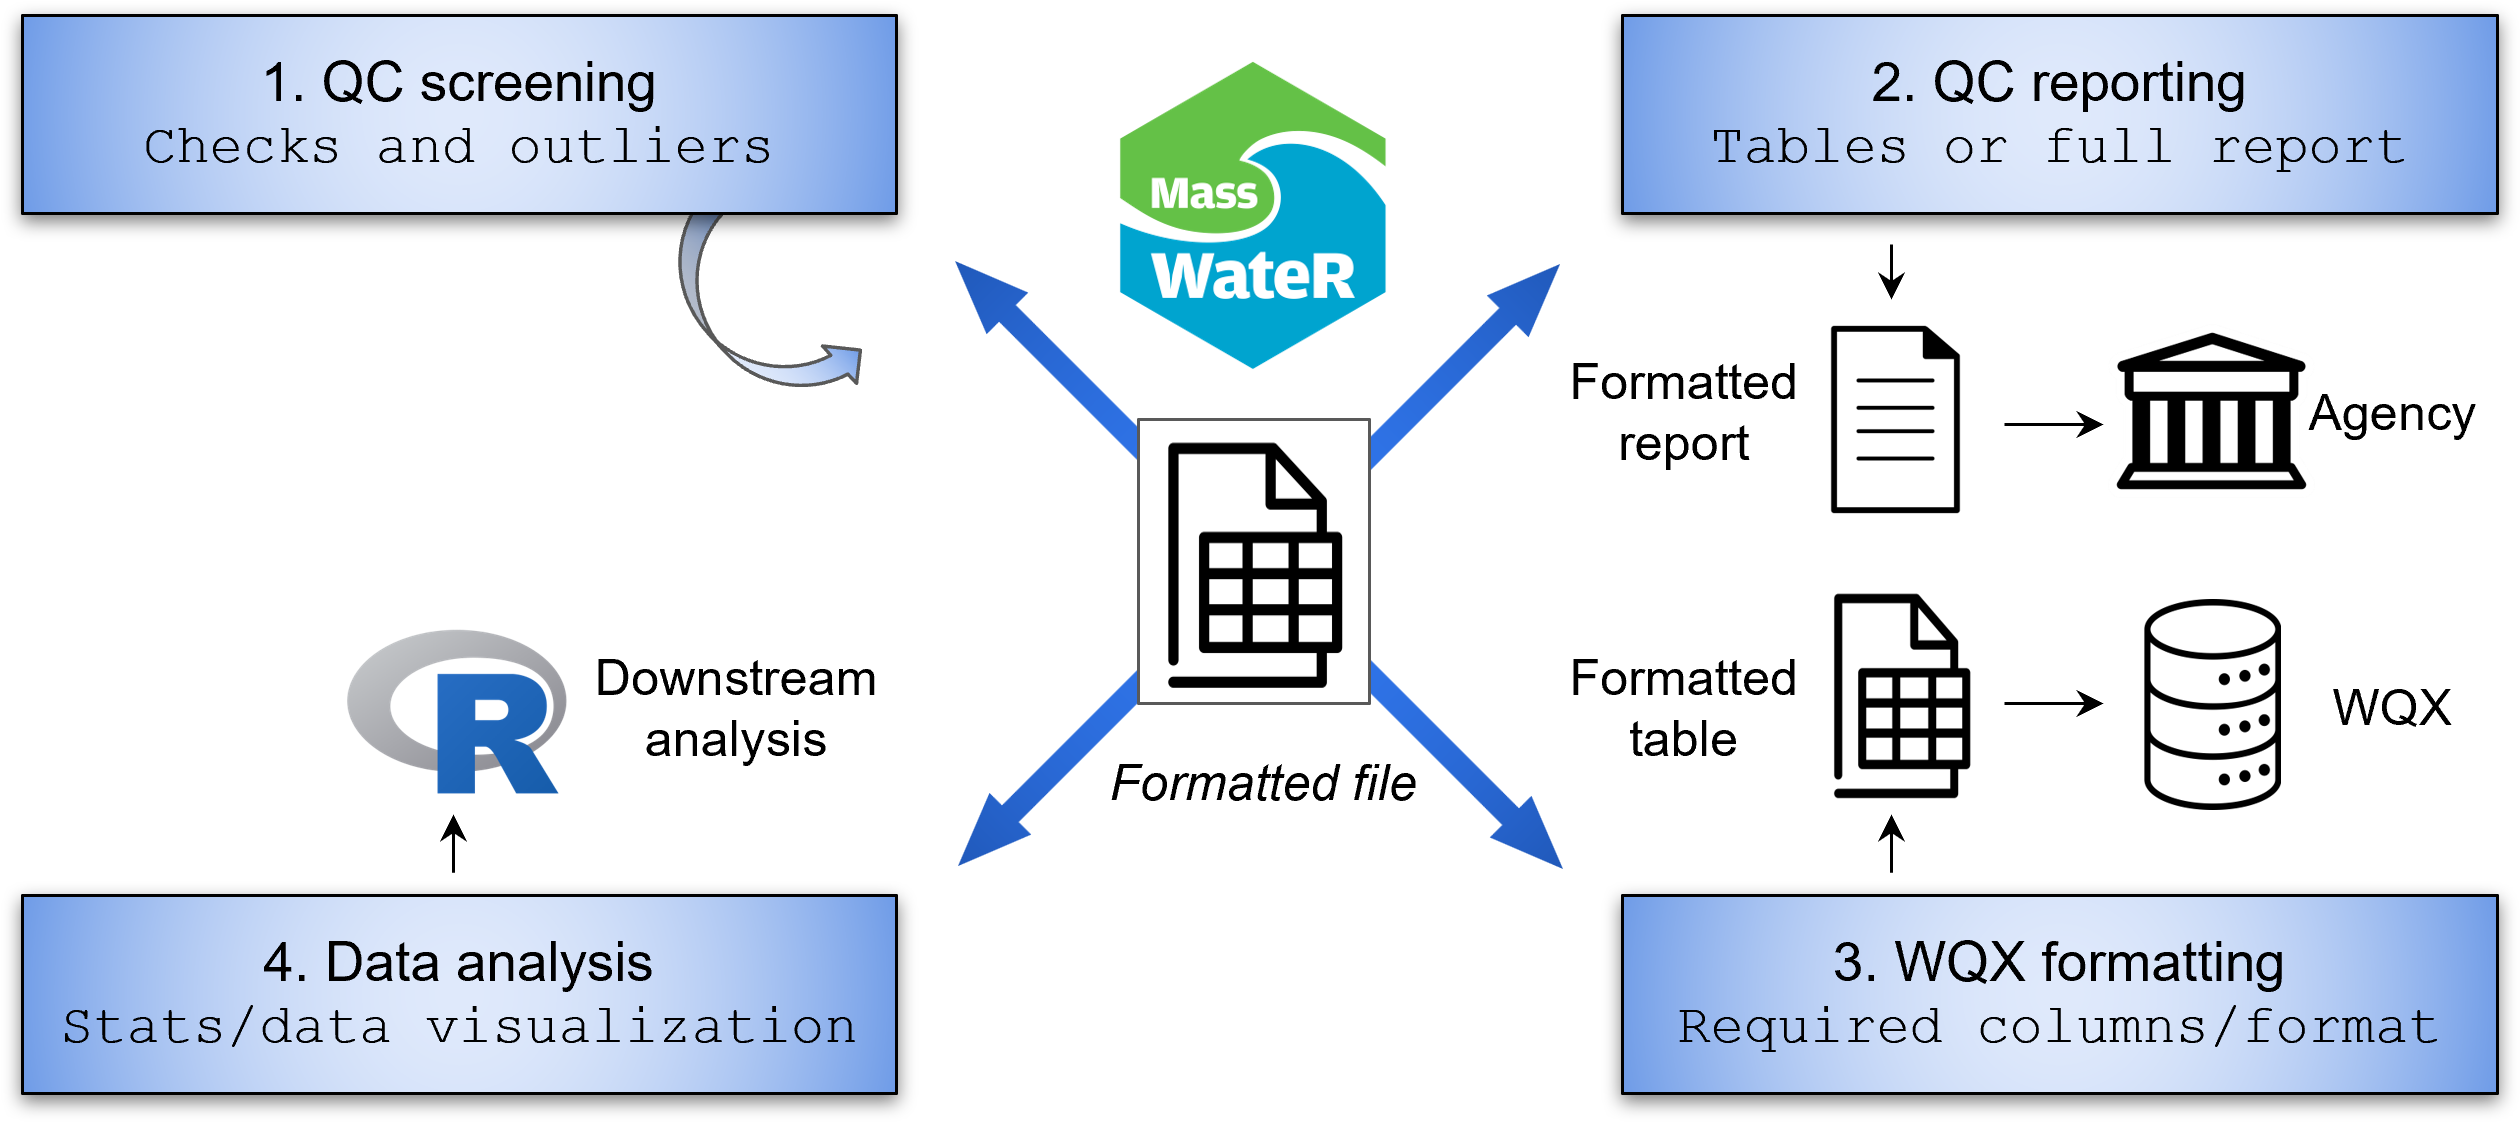
\includegraphics[width=1\linewidth]{figs/workflow} \caption{Workflow demonstrating how a user could engage with the \CRANpkg{MassWateR} package.  A user can apply one to any of the four steps depending on their need.  The first step, QC screening, is often iterative as a user can modify parts of the raw data based on input checks or outliers.  The second step can be used to create a QC report for submission to a regulatory agency.  The third step can create a formatted table for WQX submission.  The fourth step is data analysis and visualization, using \CRANpkg{MassWateR} functions and downstream analysis with additional R packages and functions.  All steps require a formatted input file.  WQX: Water Quality Exchange; QC: Quality Control.}\label{fig:workflow}
\end{figure}

No matter the user need, all data inputs to \CRANpkg{MassWateR} must follow a strict format. Developing a workflow to accommodate data inputs from the dozens of potential users from different organizations that use different data formats would have been impractical. As such, the only limitation to using the package is to adhere to the formatting requirements for all input files. Several \href{https://massbays-tech.github.io/MassWateR/RESOURCES.html}{resources} are provided on the package web page to assist potential users in this effort. These resources included several training activities that were conducted during package development and templates demonstrating the appropriate format and rationale.

The required data files for using \CRANpkg{MassWateR} are shown in table xx, including the files that apply to the workflow steps in Figure \ref{fig:workflow}. The files are each imported into R using specific \texttt{read} functions with relevant checks, explained in the next section. These checks verify multiple requirements outlined in the template files, with informative errors or warnings returned to the console to prompt the user on the required action to remedy a formatting issue. The largest input file required for all parts of the workflow in Figure \ref{fig:workflow} is the results file. This file includes all water quality monitoring data to be used with the package. As such, the formatting requirements are the most burdensome for potential users and additional functions are available to assist with formatting.

table xx

The following sections describe the basic approach to using functions in \CRANpkg{MassWateR} for any of the processes in the workflow. The naming convention for the functions is meant to provide users with an intuitive format for understanding what each function does and the step of the workflow for which the function applies. Although there are some exceptions to this nomenclature, the general format includes a prefix for each function as follows. Each prefix also includes \texttt{MWR} to avoid namespace conflicts with other packages.

\begin{itemize}
\tightlist
\item
  \texttt{read}: Read input files
\item
  \texttt{check}: Check input files for formatting issues, used internally to the read functions
\item
  \texttt{form}: Format input files for downstream functions, used internally to the read functions once the checks have passed
\item
  \texttt{anlz}: Analyze imported data
\item
  \texttt{tab}: Create formatted tables for QC analysis
\item
  \texttt{qc}: QC functions for summarizing QC results, used internally to the table functions
\item
  \texttt{util}: Various utility functions that accomplish routine tasks, but may be useful as standalone functions
\end{itemize}

Additionally, functions may often include a suffix that describes the relevant file used as input or otherwise evaluated in a downstream function.

\begin{itemize}
\tightlist
\item
  \texttt{results}: The results input file
\item
  \texttt{acc}: The data quality objectives file for accuracy
\item
  \texttt{frecom}: The data quality objectives file for frequency and completeness
\item
  \texttt{sites}: The site metadata file
\item
  \texttt{wqx}: The WQX metadata file
\end{itemize}

\hypertarget{functions}{%
\section{\texorpdfstring{\CRANpkg{MassWateR} functions}{ functions}}\label{functions}}

\hypertarget{read-and-check-files}{%
\subsection{Read and check files}\label{read-and-check-files}}

The primary task of the \texttt{read} functions is to ensure all imported files follow the required format for the package. Excel files are the expected format for all inputs and the \texttt{read} functions use the \texttt{read\_excel} function from the \CRANpkg{readxl} package (Wickham and Bryan 2023). The \texttt{read} functions do very little other than import the file - once the file is imported it is immediately passed to one of the relevant \texttt{check} functions inside the \texttt{read} function. There are several checks for each type of input file, with the number of checks increasing based on the complexity of the input file. Each check is printed to the R console on completion, whereas an error is returned at the first instance of a failed check, at which point the function is exited. The error will typically indicate which parts of the input data need to be changed to rectify the issue, often indicating a specific cell in the Excel file that requires attention. As such, the workflow is intended to be iterative, where a user imports a file, receives an error, manually changes the input file in Excel, then imports the data again until all checks pass (Figure \ref{fig:importflow}). Again, this design was purposeful as many monitoring agencies and groups collect data differently and a standard input format for the package was the best option to accommodate potential users. This may also encourage future standardization among groups for how data are maintained to ease formatting challenges to using \CRANpkg{MassWateR}. A user only needs to format their data once to use the package.

\begin{figure}
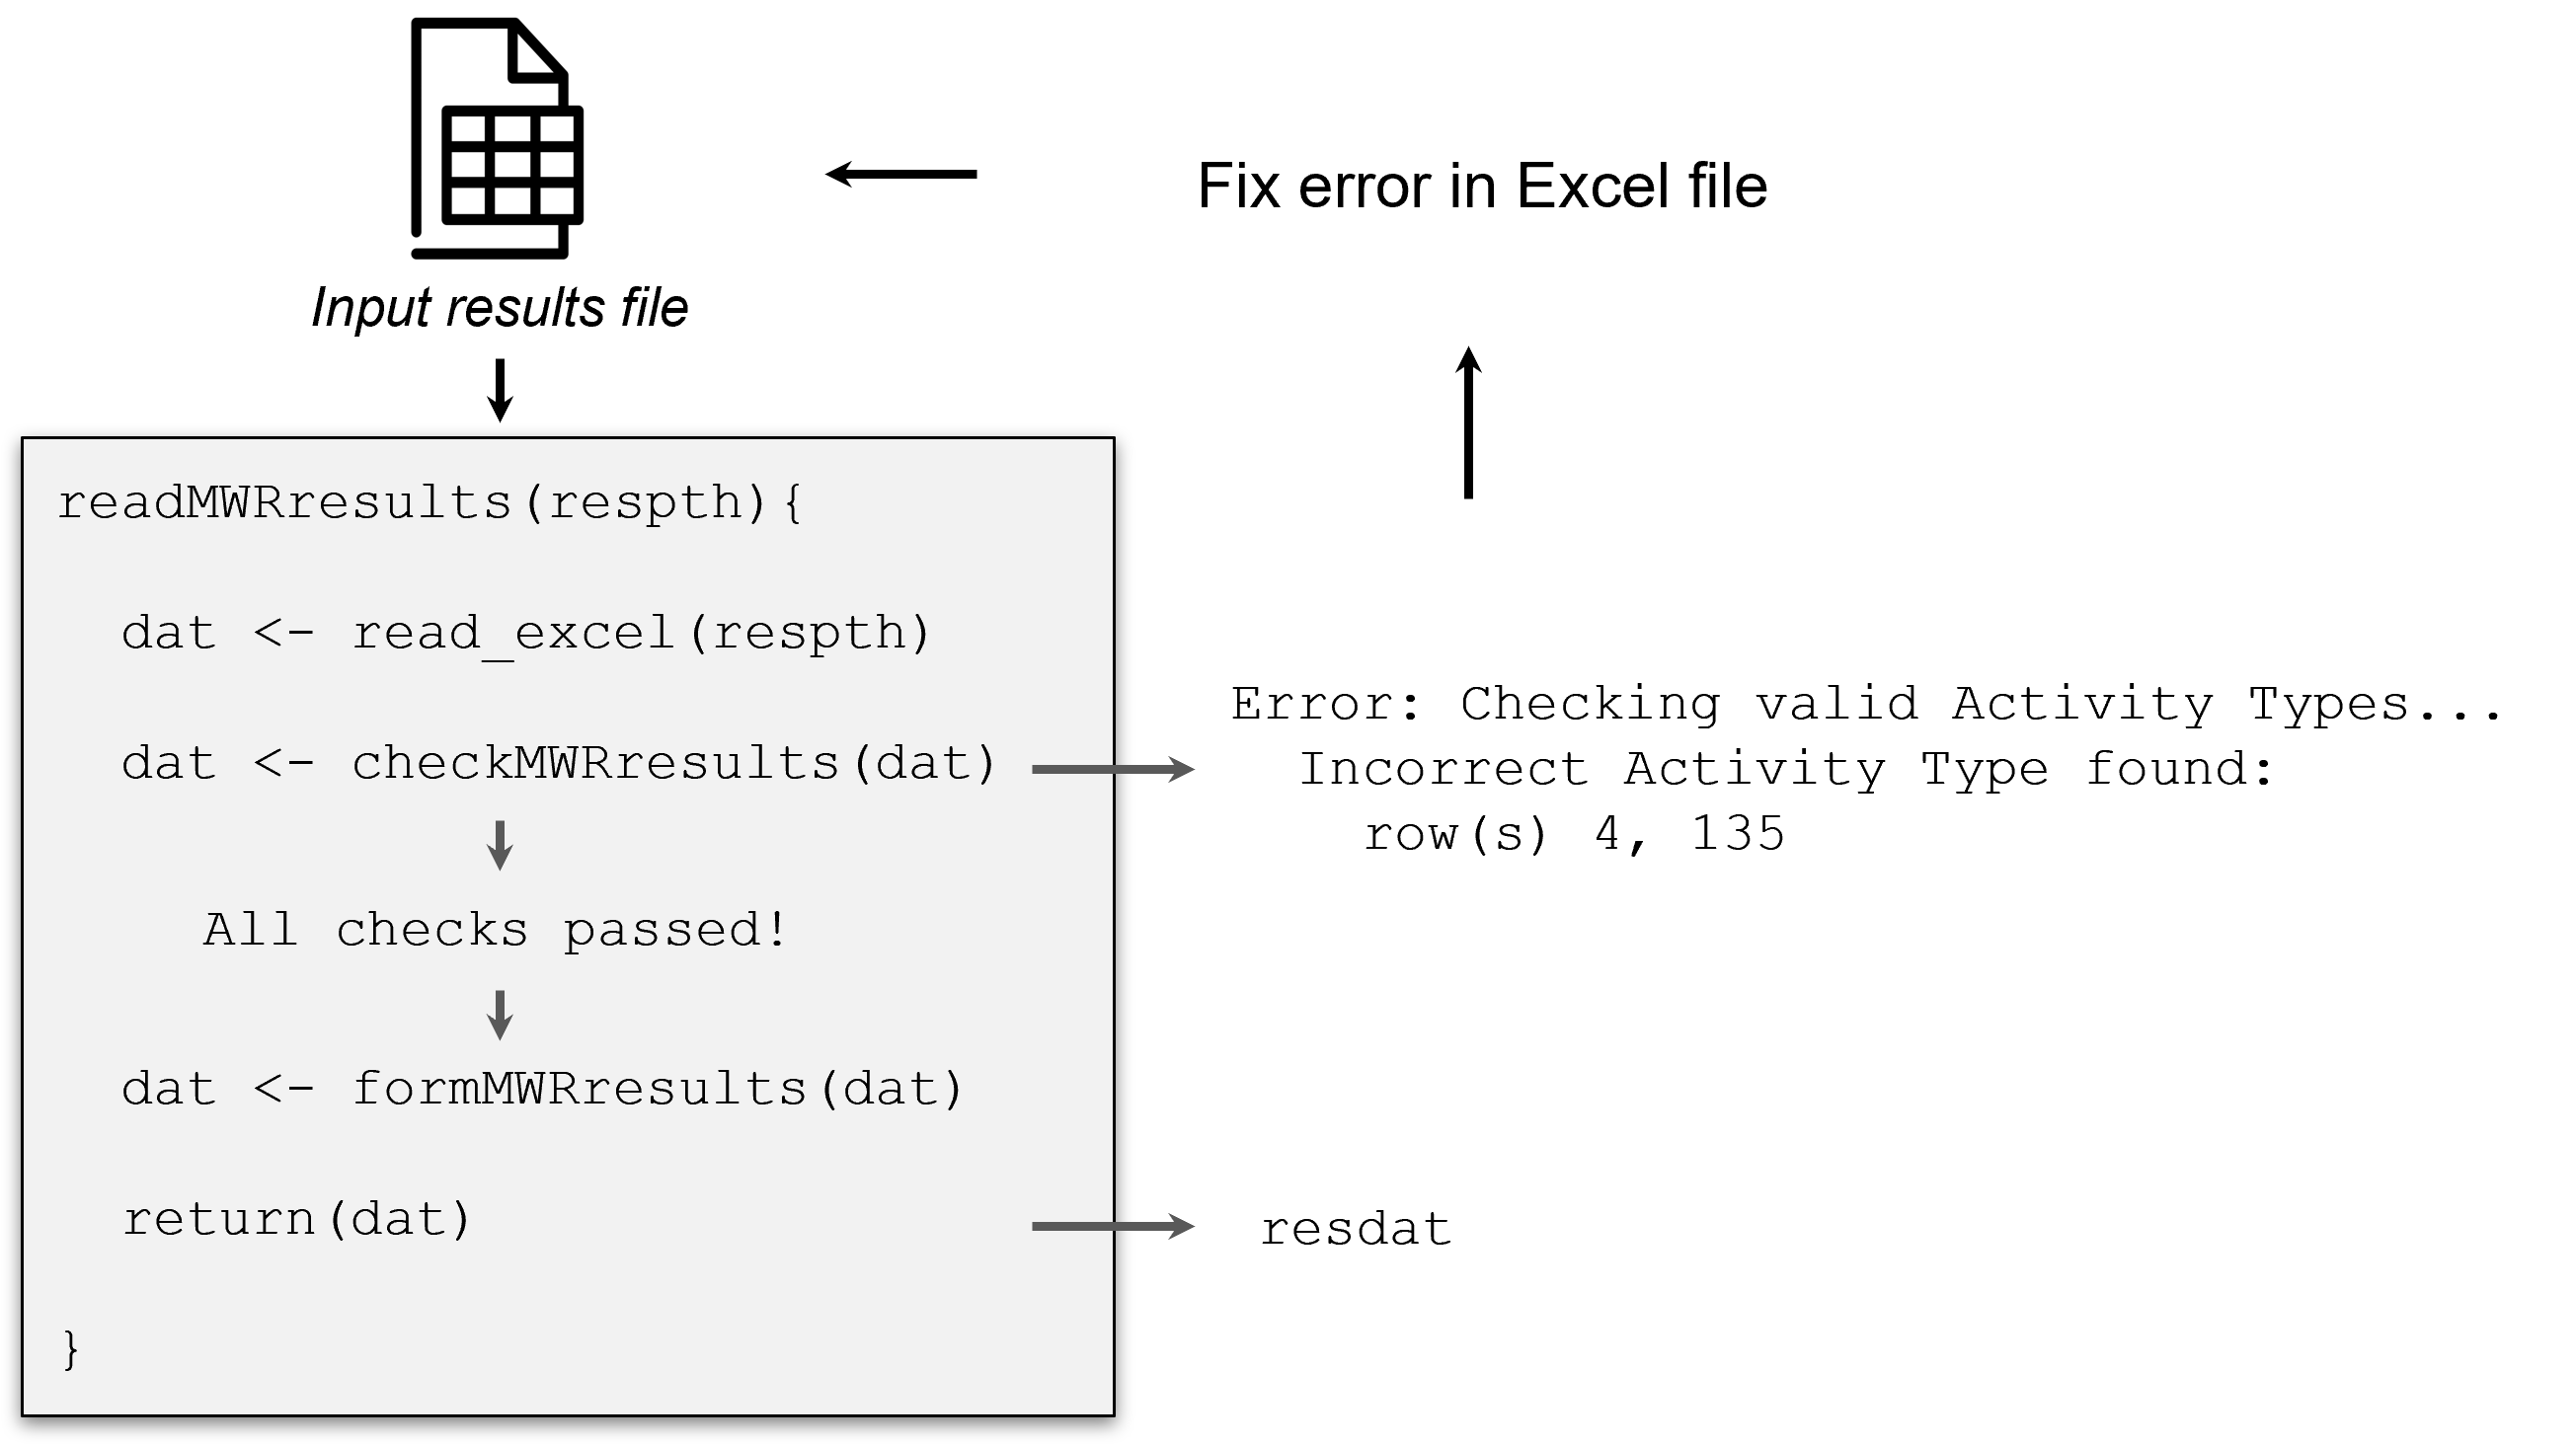
\includegraphics[width=1\linewidth]{figs/importflow} \caption{Pseudocode demonstrating the iterative process of importing a required data file for \CRANpkg{MassWateR}.  All read functions import an Excel file and the imported file is then passed to a check function.  The function exits if an error is encountered, allowing the user to manually fix the identified error and then import again.  After all checks are passed, a formatting function is applied to correct minor issues (e.g., standardize date format as YYYY-MM-DD) and the final data object is returned.}\label{fig:importflow}
\end{figure}

A correctly formatted input file would be imported as follows, with the messages in the console indicating the checks that are performed and that all checks were successful. Below demonstrates what would be shown for the results file using an example dataset included with the package. A total of fifteen checks are applied to the results file.

\begin{verbatim}
library(MassWateR)

# import results data
respth <- system.file("extdata/ExampleResults.xlsx", package = "MassWateR")
resdat <- readMWRresults(respth)
\end{verbatim}

\begin{verbatim}
#> Running checks on results data...
\end{verbatim}

\begin{verbatim}
#>  Checking column names... OK
\end{verbatim}

\begin{verbatim}
#>  Checking all required columns are present... OK
\end{verbatim}

\begin{verbatim}
#>  Checking valid Activity Types... OK
\end{verbatim}

\begin{verbatim}
#>  Checking Activity Start Date formats... OK
\end{verbatim}

\begin{verbatim}
#>  Checking depth data present... OK
\end{verbatim}

\begin{verbatim}
#>  Checking for non-numeric values in Activity Depth/Height Measure... OK
\end{verbatim}

\begin{verbatim}
#>  Checking Activity Depth/Height Unit... OK
\end{verbatim}

\begin{verbatim}
#>  Checking Activity Relative Depth Name formats... OK
\end{verbatim}

\begin{verbatim}
#>  Checking values in Activity Depth/Height Measure > 1 m / 3.3 ft... OK
\end{verbatim}

\begin{verbatim}
#>  Checking Characteristic Name formats... OK
\end{verbatim}

\begin{verbatim}
#>  Checking Result Values... OK
\end{verbatim}

\begin{verbatim}
#>  Checking QC Reference Values... OK
\end{verbatim}

\begin{verbatim}
#>  Checking for missing entries for Result Unit... OK
\end{verbatim}

\begin{verbatim}
#>  Checking if more than one unit per Characteristic Name... OK
\end{verbatim}

\begin{verbatim}
#>  Checking acceptable units for each entry in Characteristic Name... OK
\end{verbatim}

\begin{verbatim}
#> 
#> All checks passed!
\end{verbatim}

The following shows a typical error that might be returned if a check fails importing the results file. The \texttt{resdat} object is an imported results file that has passed all checks, but incorrect entries are added to the \texttt{chk} object to demonstrate the error that is returned if a user would have attempted to import this file. The \texttt{checkMWRresults()} function is run inside the \texttt{readMWRresults()} function and runs the checks (e.g., the column names are correct, all required columns are present), but then stops when invalid activity types in the \texttt{Activity\ Type} column are found. In this example, a user would need to change the entries in rows 4 and 135 of the \texttt{Activity\ Type} column in their Excel file to fix the issue and import the file again as in Figure \ref{fig:importflow}. The online \href{https://massbays-tech.github.io/MassWateR/articles/inputs.html\#data-import-and-checks}{vignette} specifies the valid entries.

\begin{verbatim}
chk <- resdat
chk[4, 2] <- "Sample"
chk[135, 2] <- "Field"
checkMWRresults(chk)
\end{verbatim}

\begin{verbatim}
#> Running checks on results data...
\end{verbatim}

\begin{verbatim}
#>  Checking column names... OK
\end{verbatim}

\begin{verbatim}
#>  Checking all required columns are present... OK
\end{verbatim}

\begin{verbatim}
#> Error:   Checking valid Activity Types...
#>  Incorrect Activity Type found: Sample, Field in row(s) 4, 135
\end{verbatim}

The \texttt{readMWRresultsview()} function is also available to assist with troubleshooting formatting issues for the results file. This function exports an Excel file that shows the unique values that are found in each column to allow a user to quickly see potential incorrect entries. The output is similar to running \texttt{apply(resdat,\ 2,\ unique)} in the console, but includes an external file that users may be more comfortable evaluating to troubleshoot formatting problems.

After all file format checks are fixed, a standard approach for using \CRANpkg{MassWateR} is to import all required files and save them as a list of named data frame objects that can be used by nearly all the package functions. This prevents the need to identify which input datasets are needed for each function, although the latter approach could used because arguments for individual input files are also provided for all functions. In the latter case, a path or data object can be used as input for each file. For the former approach, the beginning of a script for using the package could appear as follows. Example files included with the package are imported, whereas a user will specify paths to their own files.

\begin{verbatim}
library(MassWateR)

# import results data
respth <- system.file("extdata/ExampleResults.xlsx", package = "MassWateR")
resdat <- readMWRresults(respth)

# import dqo accuracy data
accpth <- system.file("extdata/ExampleDQOAccuracy.xlsx", package = "MassWateR")
accdat <- readMWRacc(accpth)

# import dqo frequency and completeness data
frecompth <- system.file("extdata/ExampleDQOFrequencyCompleteness.xlsx", package = "MassWateR")
frecomdat <- readMWRfrecom(frecompth)

# import site data
sitpth <- system.file("extdata/ExampleSites.xlsx", package = "MassWateR")
sitdat <- readMWRsites(sitpth)

# import WQX meta data
wqxpth <- system.file("extdata/ExampleWQX.xlsx", package = "MassWateR")
wqxdat <- readMWRwqx(wqxpth)

# a list of input data frames
fsetls <- list(res = resdat, acc = accdat, frecom = frecomdat, sit = sitdat, wqx = wqxdat)
\end{verbatim}

The object \texttt{fsetls} can then be used as input to downstream functions.

A final note about the data inputs is that many types of water quality measurements can be included for analysis, although the package is currently limited to working with discrete samples as compared to data from continuous monitoring equipment. The \texttt{paramsMWR} dataset included with \CRANpkg{MassWateR} provides a complete list of the parameters that can be used with the package. On data import, this list is referenced to ensure that only relevant parameters are included and that appropriate units of measurement are provided. The list includes 43 different parameters, each with multiple valid units of measurement. Additionally, only one unit of measurement is allowed per parameter, which was an intentional design so that tedious functions for converting between dozens of units of measurement did not need to be created during package development. It is not an unreasonable expectation for users to provide only one unit of measurement per parameter. Laboratories typically have a standard reporting format based on the same methodology or instrument used to measure concentrations of water quality parameters.

An additional set of functions can be used to check for outliers in the results file. Outliers can be caused by several reasons, including data entry errors, laboratory processing errors, or anomalous environmental events. Identifying and potentially removing or correcting outliers is a critical part of quality control. The functions in \CRANpkg{MassWateR} simply identify potential outliers to provide an opportunity for users to address these values. The decision on how to address outliers remains with the user and no automated tools are provided in the package to correct outliers.

The \texttt{anlzMWRoutlier()} function uses the results file and data quality objectives for accuracy to plot potential outliers by month. The accuracy file is used to automatically identify the y-axis scaling (as arithmetic or log) and to replace concentrations with appropriate values for those labelled as beyond detection. Outliers are defined using the standard definition of 1.5 times the interquartile range (the 25th to 75th percentile) of a parameter and can be visually identified as points above or below the whiskers in the boxplots. The station name for a point is also shown. The \texttt{param} specifies the water quality parameter to evaluate and the \texttt{group} argument specifies how the boxplots are grouped (by year, month, week, or station). In the following example, three stations are identified as potential outliers for the respective month.

\begin{verbatim}
anlzMWRoutlier(fset = fsetls, param = "DO", group = "month")
\end{verbatim}

\includegraphics[width=1\linewidth]{paper_files/figure-latex/unnamed-chunk-5-1}

The outliers in the above plot can also be viewed as tabular output using \texttt{outliers\ =\ TRUE} to aid in their identification.

\begin{verbatim}
anlzMWRoutlier(fset = fsetls, param = "DO", group = "month", outliers = TRUE)
\end{verbatim}

\begin{verbatim}
#> # A tibble: 3 x 6
#>   `Monitoring Location ID` `Activity Start Date` `Activity Start Time`
#>   <chr>                    <date>                <chr>                
#> 1 ELZ-004                  2022-05-15            06:50                
#> 2 HOP-011                  2022-05-15            06:55                
#> 3 ELZ-004                  2022-09-11            07:20                
#> # i 3 more variables: `Characteristic Name` <chr>, `Result Value` <dbl>,
#> #   `Result Unit` <chr>
\end{verbatim}

A user can also evaluate outliers for every water quality parameter in the results file. The \texttt{anlzMWRoutlierall()} function creates a Word document with images of boxplots for every parameter created with \texttt{anlzMWRoutlier()}. Images for each parameter can also be created as standalone files. The \texttt{param} argument does not need to be specified because all parameters are identified in the results file and processed accordingly. The following shows how to use the function by creating a single Word file or individual image files in the working directory.

\begin{verbatim}
# create word output
anlzMWRoutlierall(fset = fsetls, group = 'month', format = 'word', output_dir = getwd())

# create png output
anlzMWRoutlierall(fset = fsetls, group = 'month', format = 'png', output_dir = getwd())
\end{verbatim}

As in Figure \ref{fig:importflow}, a user can identify outliers from the results, modify the file in Excel, and import the file again for further QC reporting or analysis.

\hypertarget{quality-control-reporting}{%
\subsection{Quality Control reporting}\label{quality-control-reporting}}

The quality control functions in \CRANpkg{MassWateR}

\hypertarget{analysis}{%
\subsection{Analysis}\label{analysis}}

\hypertarget{data-submission}{%
\subsection{Data submission}\label{data-submission}}

\hypertarget{building-a-community-and-future-work}{%
\section{Building a community and future work}\label{building-a-community-and-future-work}}

All developers hope that their package is used by the intended audience. To ensure this for \CRANpkg{MassWateR}, a community of practice was\ldots{}

Building the community of practice\ldots{}

MassWater in other locations, expansion elsewhere

Inclusion of historical data

Inclusion for continuous monitoring data, consider outlier anlaysis, drift, biofouling, etc.

\hypertarget{summary}{%
\section{Summary}\label{summary}}

\hypertarget{acknowledgments}{%
\section{Acknowledgments}\label{acknowledgments}}

\hypertarget{references}{%
\section*{References}\label{references}}
\addcontentsline{toc}{section}{References}

\hypertarget{refs}{}
\begin{CSLReferences}{1}{0}
\leavevmode\vadjust pre{\hypertarget{ref-Allaire23}{}}%
Allaire, JJ, Yihui Xie, Christophe Dervieux, Jonathan McPherson, Javier Luraschi, Kevin Ushey, Aron Atkins, et al. 2023. \emph{Rmarkdown: Dynamic Documents for r}. \url{https://github.com/rstudio/rmarkdown}.

\leavevmode\vadjust pre{\hypertarget{ref-Arndt22}{}}%
Arndt, Julia, Julia S Kirchner, Kevin S Jewell, Michael P Schluesener, Arne Wick, Thomas A Ternes, and Lars Duester. 2022. {``Making Waves: Time for Chemical Surface Water Quality Monitoring to Catch up with Its Technical Potential.''} \emph{Water Research} 213: 118168. \url{https://doi.org/10.1016/j.watres.2022.118168}.

\leavevmode\vadjust pre{\hypertarget{ref-Behmel16}{}}%
Behmel, Sonja, Mathieu Damour, Ralf Ludwig, and MJ Rodriguez. 2016. {``Water Quality Monitoring Strategies---a Review and Future Perspectives.''} \emph{Science of the Total Environment} 571: 1312--29. \url{https://doi.org/10.1016/j.scitotenv.2016.06.235}.

\leavevmode\vadjust pre{\hypertarget{ref-Buytaert14}{}}%
Buytaert, Wouter, Zed Zulkafli, Sam Grainger, Luis Acosta, Tilashwork C Alemie, Johan Bastiaensen, Bert De Bièvre, et al. 2014. {``Citizen Science in Hydrology and Water Resources: Opportunities for Knowledge Generation, Ecosystem Service Management, and Sustainable Development.''} \emph{Frontiers in Earth Science} 2: 26. \url{https://doi.org/10.3389/feart.2014.00026}.

\leavevmode\vadjust pre{\hypertarget{ref-DeCicco22}{}}%
De Cicco, Laura A., David Lorenz, Robert M. Hirsch, William Watkins, and Mike Johnson. 2022. \emph{dataRetrieval: R Packages for Discovering and Retrieving Water Data Available from u.s. Federal Hydrologic Web Services} (version 2.7.12). Reston, VA: U.S. Geological Survey; U.S. Geological Survey. \url{https://doi.org/10.5066/P9X4L3GE}.

\leavevmode\vadjust pre{\hypertarget{ref-Kelly22}{}}%
Kelly-Quinn, M, JN Biggs, S Brooks, P Fortuño, S Hegarty, JI Jones, and F Regan. 2022. {``Opportunities, Approaches and Challenges to the Engagement of Citizens in Filling Small Water Body Data Gaps.''} \emph{Hydrobiologia}, 1--21. \url{https://doi.org/10.1007/s10750-022-04973-y}.

\leavevmode\vadjust pre{\hypertarget{ref-Kumpel20}{}}%
Kumpel, Emily, Clara MacLeod, Kara Stuart, Alicea Cock-Esteb, Ranjiv Khush, and Rachel Peletz. 2020. {``From Data to Decisions: Understanding Information Flows Within Regulatory Water Quality Monitoring Programs.''} \emph{Npj Clean Water} 3 (1): 38. \url{https://doi.org/10.1038/s41545-020-00084-0}.

\leavevmode\vadjust pre{\hypertarget{ref-Schiff16}{}}%
Schiff, Ken, PR Trowbridge, ET Sherwood, Peter Tango, and Rich A Batiuk. 2016. {``Regional Monitoring Programs in the United States: Synthesis of Four Case Studies from Pacific, Atlantic, and Gulf Coasts.''} \emph{Regional Studies in Marine Science} 4: A1--7. \url{https://doi.org/10.1016/j.rsma.2015.11.007}.

\leavevmode\vadjust pre{\hypertarget{ref-Stein09}{}}%
Stein, Eric D, and Donald B Cadien. 2009. {``Ecosystem Response to Regulatory and Management Actions: The Southern California Experience in Long-Term Monitoring.''} \emph{Marine Pollution Bulletin} 59 (4-7): 91--100. \url{https://doi.org/10.1016/j.marpolbul.2009.02.025}.

\leavevmode\vadjust pre{\hypertarget{ref-Tango13}{}}%
Tango, Peter J, and Richard A Batiuk. 2013. {``Deriving {C}hesapeake {B}ay Water Quality Standards.''} \emph{JAWRA Journal of the American Water Resources Association} 49 (5): 1007--24. \url{https://doi.org/10.1111/jawr.12108}.

\leavevmode\vadjust pre{\hypertarget{ref-Wickham16}{}}%
Wickham, Hadley. 2016. \emph{Ggplot2: Elegant Graphics for Data Analysis}. Springer-Verlag New York. \url{https://ggplot2.tidyverse.org}.

\leavevmode\vadjust pre{\hypertarget{ref-Wickham23}{}}%
Wickham, Hadley, and Jennifer Bryan. 2023. \emph{Readxl: Read Excel Files}. \url{https://CRAN.R-project.org/package=readxl}.

\leavevmode\vadjust pre{\hypertarget{ref-Wilde02}{}}%
Wilde, Franceska D., and U.S. Geological Survey. 2002. {``Chapter A5. Processing of Water Samples.''} Techniques of Water-Resources Investigations 09-A5. Version 2.2, Revised February 2009. Reston, VA: U.S. Geological Survey. \url{https://doi.org/10.3133/twri09A5}.

\leavevmode\vadjust pre{\hypertarget{ref-Xie15}{}}%
Xie, Yihui. 2015. \emph{Dynamic Documents with {R} and Knitr}. 2nd ed. Boca Raton, Florida: Chapman; Hall/CRC. \url{https://yihui.org/knitr/}.

\end{CSLReferences}

\bibliography{RJreferences.bib}

\address{%
Marcus W. Beck\\
Tampa Bay Estuary Program\\%
263 13th Ave S\\ St.~Petersburg, Florida, USA 33701\\
%
\url{https://tbep.org}\\%
\textit{ORCiD: \href{https://orcid.org/0000-0002-4996-0059}{0000-0002-4996-0059}}\\%
\href{mailto:mbeck@tbep.org}{\nolinkurl{mbeck@tbep.org}}%
}

\address{%
Benjamen Wetherill\\
ACASAK Consulting\\%
Boston, Massachusetts, USA\\
%
\url{https://www.acasak.com/}\\%
\textit{ORCiD: \href{https://orcid.org/0000-0002-0912-0225}{0000-0002-0912-0225}}\\%
\href{mailto:bwetherill@acasak.co}{\nolinkurl{bwetherill@acasak.co}}%
}

\address{%
Jillian Carr\\
Massachusetts Bays National Estuary Partnership\\%
University of Massachusetts Boston, 100 Morrissey Blvd\\ Boston, Massachusetts, USA 02125\\
%
\url{https://www.mass.gov/orgs/massachusetts-bays-national-estuary-partnership}\\%
%
\href{mailto:Jillian.Carr@umb.edu}{\nolinkurl{Jillian.Carr@umb.edu}}%
}

\address{%
Pamela DiBona\\
Massachusetts Bays National Estuary Partnership\\%
University of Massachusetts Boston, 100 Morrissey Blvd\\ Boston, Massachusetts, USA 02125\\
%
\url{https://www.mass.gov/orgs/massachusetts-bays-national-estuary-partnership}\\%
%
\href{mailto:pamela.dibona@state.ma.us}{\nolinkurl{pamela.dibona@state.ma.us}}%
}
